% 
% Lecture Template for ME3023 -  Measurements in Mechanical Systems - Tennessee Technological University
%
% Spring 2020 - Summer 2020
% Tristan Hill, May 07, 2020 - June 12, 2020 - July 08, 2020
% Module 6->4 - Steady State Circuits
% Topic 2 - Fundamental Laws
%


\documentclass[fleqn]{beamer} % for presentation (has nav buttons at bottom)

\usepackage{/home/thill/Documents/lectures/measurements_lectures/measurements_lectures}

%\newcommand{\MNUM}{4\hspace{2mm}} % Module number
\newcommand{\TNUM}{2\hspace{2mm}} % Topic number 
\newcommand{\moduletitle}{Steady State Circuits}
\newcommand{\topictitle}{Fundamental Laws} 

\newcommand{\sectiontitleI}{Ohm's Law}
\newcommand{\sectiontitleII}{Combining Resistance}
\newcommand{\sectiontitleIII}{Kirchhoff's Laws}
\newcommand{\sectiontitleIV}{Power Dissipation}

% custom box
\newsavebox{\mybox}

\title{Lecture Module - \moduletitle}

\date{Mechanical Engineering\vspc Tennessee Technological University}

\begin{document}
	
	\lstset{language=MATLAB,basicstyle=\ttfamily\small,showstringspaces=false}
	
	\frame{\titlepage \center\begin{framed}\Large \textbf{Topic \TNUM - \topictitle}\end{framed} \vspace{5mm}}


% Section 0: Outline
\frame{

\large \textbf{Topic \TNUM - \topictitle} \vspace{3mm}\\


\begin{itemize}

	\item \sectiontitleI    \vspc % Section I
	\item \sectiontitleII 	\vspc % Section II
	\item \sectiontitleIII 	\vspc %Section III
	\item \sectiontitleIV 	\vspc %Section IV

\end{itemize}

}

% Section I:
\section{\sectiontitleI}

% Section I - Frame I:
\frame{ \small
\frametitle{\sectiontitleI}

\begin{multicols}{3}

{\bf James Maxwell}
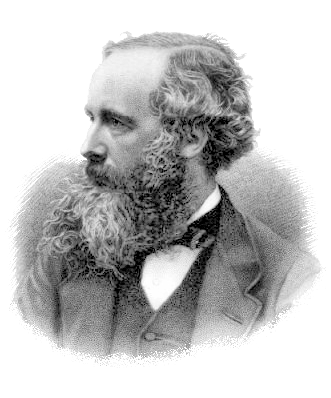
\includegraphics[scale=.30]{James_Clerk_Maxwell.png} \hspace{3mm}	

{\bf George Ohm} 
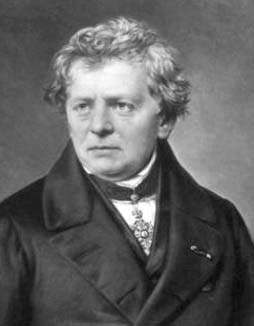
\includegraphics[scale=.30]{George_Ohm.png}	

{\bf Ohm's Notebook}
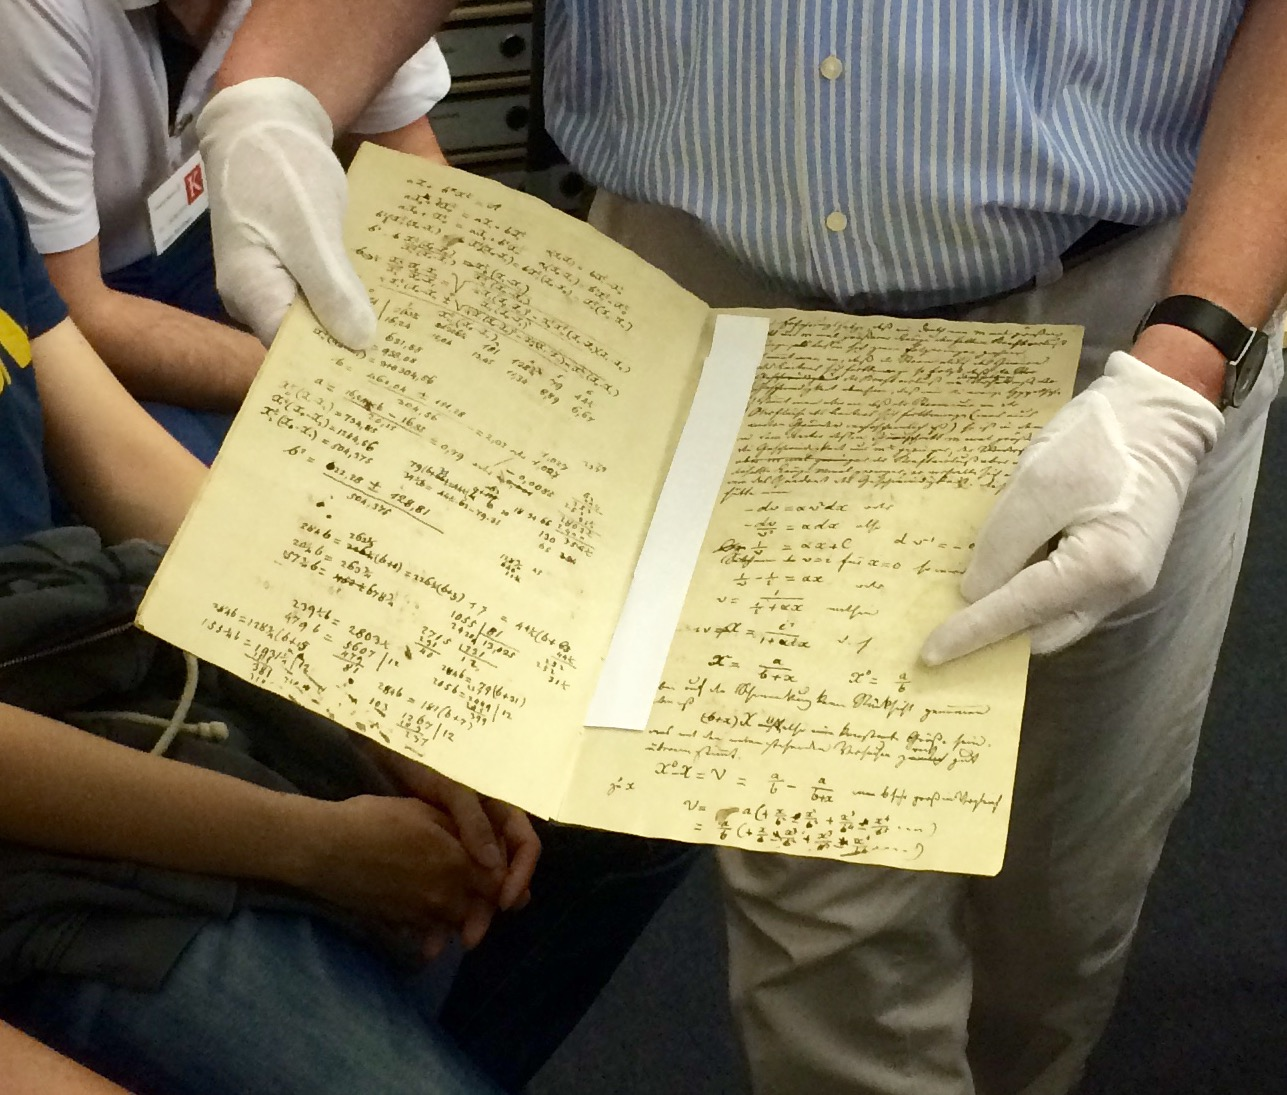
\includegraphics[scale=.07]{Ohms_Laborbuch.jpg}	

\end{multicols}
Ohm did his work on resistance in the years 1825 and 1826, and published his results in 1827 as the book Die galvanische Kette, mathematisch bearbeitet...
}

% Section I - Frame II:
\frame{ \small
\frametitle{\sectiontitleI}
Ohm's law states that the current through a conductor between two points is directly proportional to the voltage across the two points. \vspace{15mm}

\begin{multicols}{2}

 
It is more commonly shown in the following form.


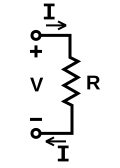
\includegraphics[scale=.8]{OhmsLaw.png}

\end{multicols}

}


% Section II:
\section{\sectiontitleII}

% Section II - Frame I:
\frame{
\frametitle{\sectiontitleII}
\begin{multicols}{2}

\begin{center}
Resistors in Series\vspcc
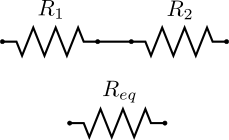
\includegraphics[scale=.2]{series_resistors.png} 
\end{center}

\vspace{15mm}

\begin{center}
Resistors in Parallel \vspcc
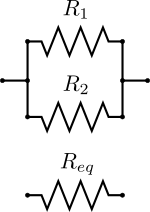
\includegraphics[scale=.2]{parallel_resistors.png}
\end{center}

\vspace{10mm}

\end{multicols}

}


% Section III:
\section{\sectiontitleIII}

% Section III - Frame I:
\frame{ \small
\frametitle{\sectiontitleIII}

Both of Kirchhoff's laws can be understood as corollaries of Maxwell's equations in the low-frequency limit. They are accurate for DC circuits, and for AC circuits at frequencies where the wavelengths of electromagnetic radiation are very large compared to the circuits. \vspc 

\begin{enumerate}
\item Kichhoff's Voltage Law (KVL)
\item Kichhoff's Current  Law (KCL)
\end{enumerate}

}

% Section III - Frame II:
\frame{ \small
\frametitle{\sectiontitleIII}

\begin{multicols}{2}
{\bf Kichhoff's Voltage Law (KVL)} - The sum of the voltages around a loop (aka mesh) equals zero.\\ 
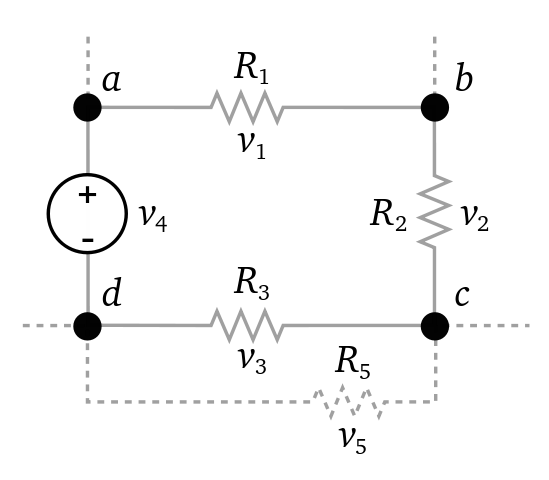
\includegraphics[scale=.20]{Kirchhoffs_voltage_law.png} 

{\bf Kichhoff's Current  Law (KCL)} - The sum of the current flowing in and out of  node (aka junction) equals zero.  \vspace{2mm}\\
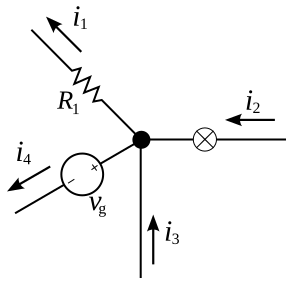
\includegraphics[scale=.4]{Kirchhoffs_current_law.png} 
\end{multicols}

}

%% Section IV:
\section{\sectiontitleIV}

% Section IV - Frame I:
\frame{ \small
\frametitle{\sectiontitleIV}
	Energy is transformed in to heat in passive circuit components. For a resistor the power dissipation can be found with following relations. \vspace{5mm}
	
	
}
	
% Section IV - Frame II:
\frame{ \small
\frametitle{\sectiontitleIV}

	Power is the rate of energy dissipated, aka the amount of energy lost per unit of time. How do we compute total energy for the power? 
	
  
}


\end{document}





